\documentclass{article}[10pt]
\usepackage[utf8]{inputenc}

\title{Sistemas Digitais}
\author{Paula Oliveira}
\date{October 2018}

\usepackage{natbib}
\usepackage{graphicx}

\begin{document}

\maketitle

\section{Introdução}
O curso de Sistemas Digitais almeja que os seus alunos construam conhecimento sobre circuitos lógicos digitais combinacionais e sequenciais que abrangem circuitos digitais de pequena complexidade até circuitos de média complexidade. Os alunos desta cadeira, têm a experiência de desenvolver todo o fluxo de projeto, desde de sua especificação, através do Quartus II, até sua implementação.

\begin{figure}[h!]
\centering
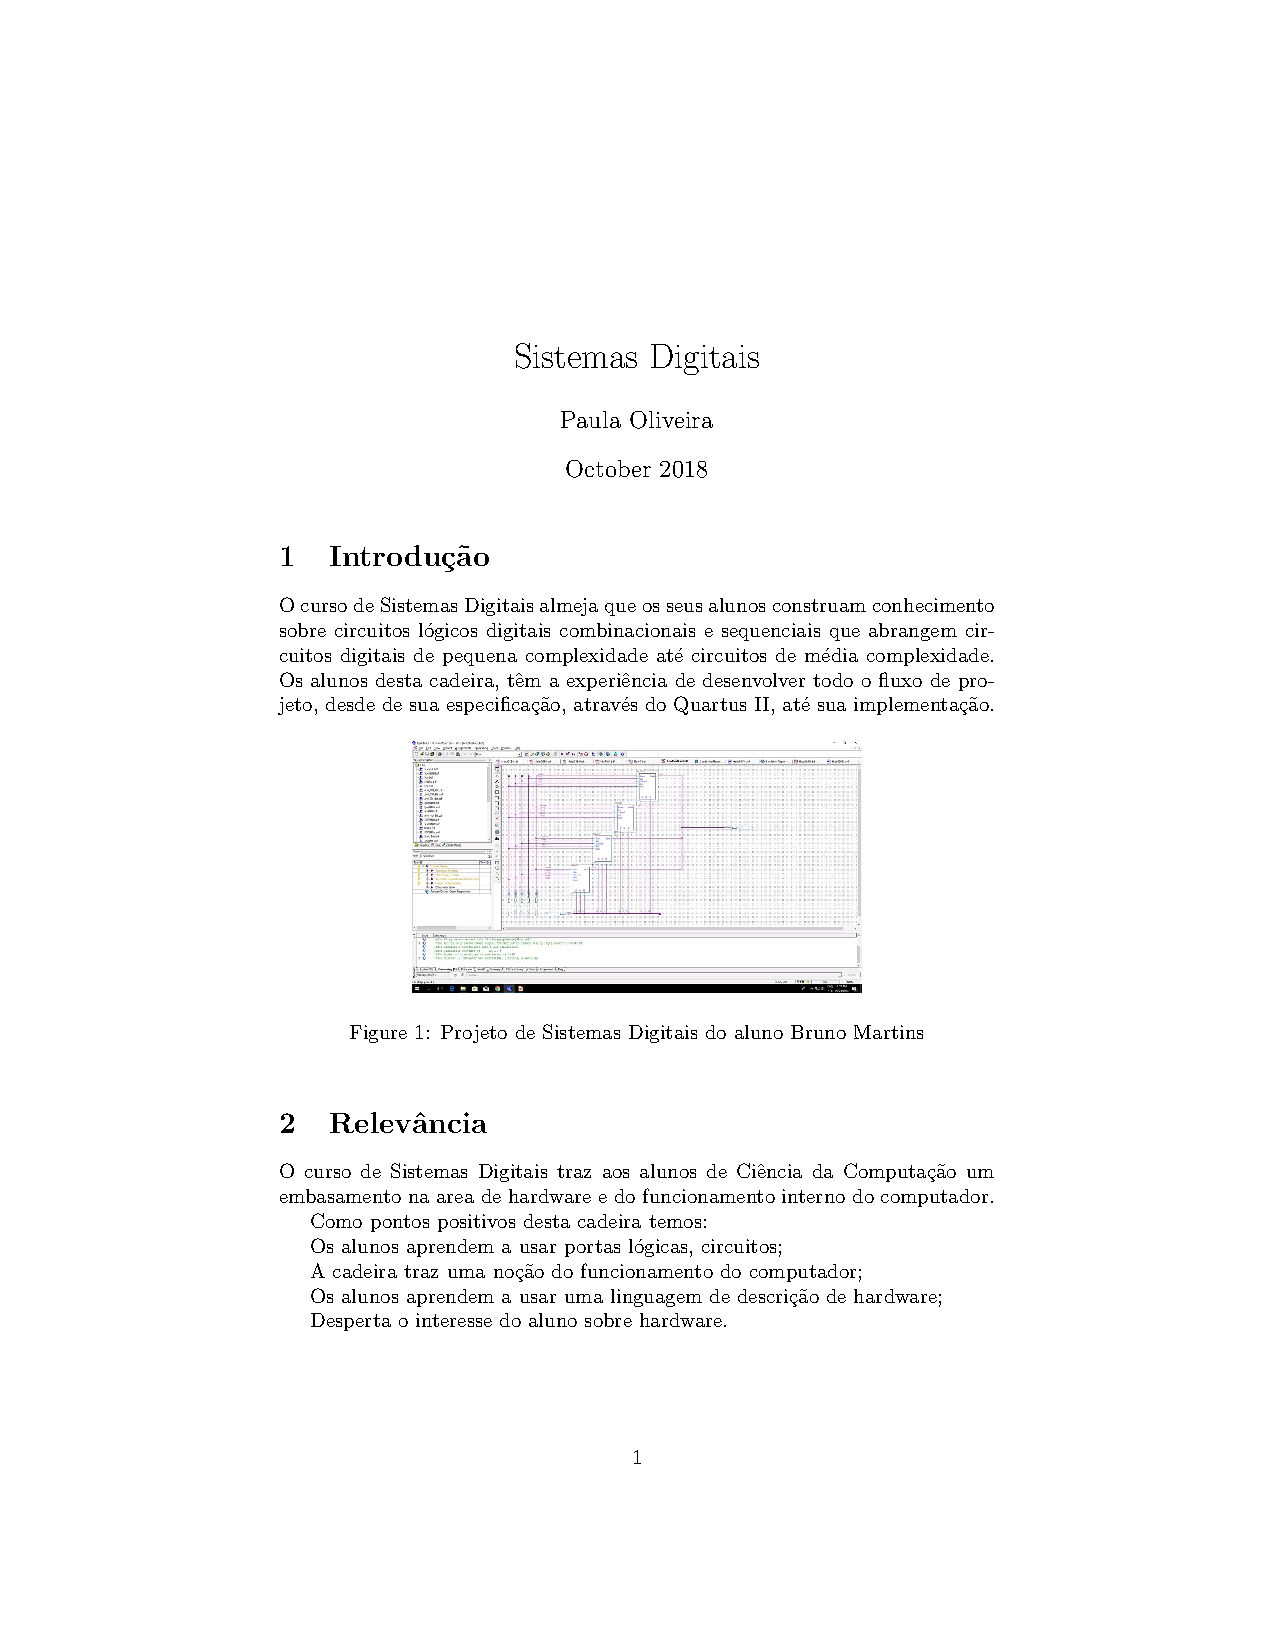
\includegraphics[scale=0.2]{pcos.jpg}
\caption{Projeto de Sistemas Digitais do aluno Bruno Martins}
\label{fig:universe}
\end{figure}

\section{Relevância}
O curso de Sistemas Digitais traz aos alunos de Ciência da Computação um embasamento na area de hardware e do funcionamento interno do computador.

Como pontos positivos desta cadeira temos:

Os alunos aprendem a usar portas lógicas, circuitos;

A cadeira traz uma noção do funcionamento do computador;

Os alunos aprendem a usar uma linguagem de descrição de hardware;

Desperta o interesse do aluno sobre hardware.

 
 
 \section{Relação com outras disciplinas}
 \begin{tabular}{c|cl}

  Disciplina   & Descrição \\\hline
  \\
   infraestrutura de hardware  & Tem como objetivo, instruir os alunos sobre: processadores, \\& sistema de memória, entradas e saída e barramentos. \\&  Neste curso, os princípios de fundamento de cada um desses \\& componentes são explorados. \\\hline
   \\
   Tópicos avançados em \\Robótica e Automação Inteligente &  Estudo de técnicas avançadas em na área multidisciplinar \\& de Robótica e Automação Inteligente permitindo \\& ao aluno conhecer o estado da\\& arte nesta área de pesquisa.
\end{tabular}

\bibliographystyle{plain}
\bibliography{references}
    As referências utilizadas neste texto foram os sites {link: SistemasDigitais}, {link: InfraDeHardare}, {link: Robotica}
\end{document}
